% Tamaño de letra.
\documentclass[12pt,titlepage]{article}

%------------------------------ Paquetes ----------------------------------

% Paquetes:
 
%Para comentarios multilínea.
\usepackage{verbatim}

% Para tener cabecera y pie de página con un estilo personalizado.
\usepackage{fancyhdr}

% Codificación UTF-8
\usepackage[utf8]{inputenc}

% Castellano.
\usepackage[spanish]{babel}

% Tamaño de página y márgenes.
\usepackage[a4paper,headheight=16pt,scale={0.75,0.8},hoffset=0.5cm]{geometry}

% Para poder agregar notas al pie en tablas:
%\usepackage{threeparttable}

% Tipo de letra Helvetica (Arial).
%\usepackage{helvet}
%\renewcommand\familydefault{\sfdefault}

% Gráficos:

% Para incluir imágenes, el siguiente código carga el paquete graphicx
% según se esté generando un archivo dvi o un pdf (con pdflatex).

% Para generar dv.
%\usepackage[dvips]{graphicx}

% Para generar pdf.
\usepackage[pdftex]{graphicx}
\pdfcompresslevel=9

\usepackage{appendix}
\usepackage{pdfpages}
\usepackage{longtable}
\usepackage{url}


%
% Directorio donde están las imagenes.
%
%\newcommand{\imgdir}{includes}
%\graphicspath{{\imgdir/}}

%------------------------------ ~paquetes ---------------------------------

%------------------------- Inicio del documento ---------------------------

\begin{document}

% ---------------------- Encabezado y pie de página -----------------------

% Encabezado: sección a la derecha.
% Pie de página: número de página a la derecha.

\pagestyle{fancy}
\renewcommand{\sectionmark}[1]{\markboth{}{\thesection\ \ #1}}
\lhead{}
\chead{}
\rhead{\rightmark}
\lfoot{}
\cfoot{}
\rfoot{\thepage}

% ---------------------- ~Encabezado y pie de página ----------------------

% -------------------------- Título y autor(es) ---------------------------

\title{ConcuShare}
\author{}

% -------------------------- ~Título y autor(es) --------------------------

% ------------------------------- Carátula --------------------------------

\begin{titlepage}

\thispagestyle{empty}

% Logo facultad más pie de la figura.
\begin{center}

\includegraphics[scale=0.55]{./Images/fiuba}\\
\large{\textsc{Universidad de Buenos Aires}}\\
\large{\textsc{Facultad De Ingeniería}}\\
\small{Año 2012 - 1\textsuperscript{er} Cuatrimestre}
\end{center}

\vfill

% Título central.
\begin{center}

\Large{\underline{\textsc{Sistema de Programaci\'on No Convencional de Robots}}}
\Large{\underline{\textsc{(75.70)}}}

\vfill

% Tabla de integrantes.

\Large{\underline{\textsc{Trabajo Pr\'actico Final}}} \\
\Large{\underline{\textsc{El juego Ta-Te-Ti}}}
\vfill
 
\Large\underline{Integrantes} \linebreak\linebreak

% Separación entre columnas.
\large\addtolength{\tabcolsep}{-3pt}
% Tres columnas con alineación centrada.
\begin{tabular}{|| c | c | c ||}
\hline
\textbf{Apellido, Nombre} & \textbf{Nro. Padrón} & \textbf{E-mail} \\
\hline
Bukaczewski, Verónica & 86954 & vero13@gmail.com \\
\hline
Rivero, Hern\'an & 88455 & riverohernanj@gmail.com \\
\hline
\end{tabular}
\end{center}

\vfill

\hrule
\vspace{0.2cm}

% Pie de página de la carátula.
%\noindent\small{75.70 - Sistema de Programaci\'on No Convencional de Robots \hfill}

\end{titlepage}

% ------------------------------- ~Carátula -------------------------------

% ----------------------- Cabeceras y pies de página ----------------------

\pagestyle{fancy}
\lhead{}
\chead{}
\rhead{}
\lfoot{\scriptsize{75.70 - Sistema de Programaci\'on No Convencional de Robots \\
\\Trabajo práctico Final - 1er cuatrimestre 2012}}
\cfoot{}
\rfoot{\\\thepage}
\renewcommand{\headrulewidth}{0pt}

% ---------------------- ~Cabeceras y pies de página ----------------------

% -------------------------------- Índice ---------------------------------

% Hago que las páginas se comiencen a contar a partir de aquí.
\setcounter{page}{2}

% Índice.
\newpage
\thispagestyle{empty}
\tableofcontents
\newpage

% -------------------------------- ~Índice --------------------------------

% ----------------------------- Inicio del tp -----------------------------

\section{Objetivo}
El objetivo del presente trabajo pr\'actico es entrenar una red neuronal para que juegue al Ta-Te-Ti. Se utilizar\'a una red neuronal de tipo backpropagation, para generar un m\'etodo de aprendizaje a medida que se desarrollan las partidas de Ta-Te-Ti.

\section{El juego Ta-Te-Ti}
Por lo general, el Ta-Te-Ti se juega en una cuadrícula de tres por tres (ver Figura [\ref{grilla-vacia}]). Cada jugador, a su vez se mueve mediante la colocación de un marcador en un casillero vac\'io. El marcador de un jugador es ``X``(cruz) y el del otro es ``O``(c\'irculo). El juego termina tan pronto como un jugador tiene tres marcadores en una fila: horizontalmente, verticalmente, o en diagonal (un ejemplo se muestra en la Figura [\ref{cruz-gana}]). El juego puede también terminan en empate (ver Figura [\ref{empate-tateti}]), si no hay posibilidad de ganar para alguno de los jugadores.

\begin{figure}[h!]
 \centering
 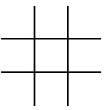
\includegraphics{./Images/grilla-tateti.png}
 % grilla-tateti.png: 104x110 pixel, 96dpi, 2.75x2.91 cm, bb=0 0 78 82
 \caption{Grilla vac\'ia TaTeTi.}
 \label{grilla-vacia}
\end{figure}

\begin{figure}[h!]
 \centering
 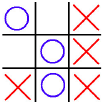
\includegraphics{./Images/cruz-gana-tateti.png}
 % cruz-gana-tateti.png: 103x105 pixel, 96dpi, 2.72x2.78 cm, bb=0 0 77 79
 \caption{El jugador cruz gana la partida.}
 \label{cruz-gana}
\end{figure}

\begin{figure}[h!]
 \centering
 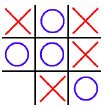
\includegraphics{./Images/empate-tateti.png}
 % empate-tateti.png: 104x109 pixel, 96dpi, 2.75x2.88 cm, bb=0 0 78 82
 \caption{La partida termin\'o empatada.}
 \label{empate-tateti}
\end{figure}


\section{Soluciones propuestas}


\section{Soluci\'on elegida}

\subsection{Estructura de la Red Neuronal}
Para el armado de la red neural, se tuvo en cuenta que la cantidad de casilleros del tablero de Ta-Te-Ti es 9 y que por cada uno se tiene la posibilidad de encontrar tres tipos de elementos (cruz, c\'irculo y vac\'io). Entonces, como primera capa oculta se decidi\'o utilizar 27 (9x3) filas. Para las siguientes capas ocultas se decidieron utilizar 9 y 3 filas, en funci\'on de la cantidad de casilleros y elementos posibles.

\subsection{Entrenando la Red Neuronal}

\subsection{Resultados}

\section{Conclusiones}


% -------------------------------- Apendice --------------------------------
\appendix
\section{Apendice}


% ------------------------------- ~Apendice -------------------------------

% ----------------------------- Bibliografia ------------------------------
\begin{thebibliography}{99}
	\bibitem{docjoone}
		\textbf{Documentaci\'on Joone} \\
		\url{http://sourceforge.net/projects/joone/files/Documentation/DTE/JooneDTEGuide.pdf}

	\bibitem{tutorialjoone}
		\textbf{Tutorial B\'asico Joone} \\
		\url{http://ubuntuone.com/p/1dB/}

	\bibitem{tic-tac-toe1}
		\textbf{Training an artificial neuronal network to play tic-tac-toe} \\
		\url{http://users.auth.gr/kehagiat/GameTheory/12CombBiblio/TicTacToe.pdf}

	\bibitem{tic-tac-toe2}
		\textbf{How to code an artificial neural network (Tic-tac-toe)?} \\
		\url{http://stackoverflow.com/questions/761216/} \\
		\url{how-to-code-an-artificial-neural-network-tic-tac-toe}

	\bibitem{tic-tac-toe3}
		\textbf{Neural Net Training for Tic-Tac-Toe} \\
		\url{www.cs.virginia.edu/~bmb5v/cs660/Project.doc}

	\bibitem{tic-tac-toe4}
		\textbf{TD Learning of Game Evaluation Functions with Hierarchical Neural Architectures} \\
		\url{http://webber.physik.uni-freiburg.de/~hon/vorlss02/Literatur/reinforcement/GameEvaluationWithNeuronal.pdf}

\end{thebibliography}

% ---------------------------- ~Bibliografia ------------------------------

% ------------------------------ Fin del tp -------------------------------

\end{document}

%---------------------------- Fin del documento ---------------------------

